

\documentclass[UTF8]{ctexart}
\usepackage{amsfonts}
\usepackage{amsmath}
\usepackage{amssymb}
\usepackage{float}
\usepackage{graphicx}
\usepackage{fancyhdr}
\pagestyle{empty}



%\usepackage{pgfplots}
%\usepgfplotslibrary{dateplot}

\title{觅食算法之布朗运动}
%\subtitle{A modern beamer theme}
\date{\today}

\author{李崇慧(学号:11704020,人文学院)}

%\titlegraphic{\hfill\includegraphics[height=1.5cm]{logo.pdf}}

\begin{document}

\maketitle


\section{随机过程与布朗运动}
我们周边充满了各种各样的数据,所谓大数据时代,这些数据最基本的特点就是含有巨量的噪音,而随机过程就是尝试从这些噪音里提取出信息。随机过程描述的是一个量随时间可能的变化,在这个过程里,每一个时刻变化的方向都是不确定的,或者说随机过程就是由一系列随机变量组成,每一个时刻系统的状态都由一个随机变量表述,而整个过程则构成态空间的一个轨迹(随机过程的实现)。


\section{布朗运动的简史}
最初由英国生物学家布朗(Brown)于1827年提出这种物理现象。1905年爱因斯坦首次对这一现象的物理规律给出数学描述。1918年维纳(Wiener)运用数学理论严格描述这种无规则运动。并用随机过程理论和概率理论建立了数学模型。因此又称为维纳过程。是具有连续时间参数和连续状态空间的一类随机过程。

自1860年以来,许多科学家都在研究此种现象,后来发现布朗运动有下列的主要特性:
\begin{itemize}
  \item 粒子的运动由平移及转移所构成,显得非常没规则而且其轨迹几乎是处处没有切线。
  \item 粒子之移动显然互不相关,甚至于当粒子互相接近至比其直径小的距离时也是如此。
  \item 粒子的成分及密度对其运动没有影响。
  \item 粒子越小或液体粘性越低或温度越高时,粒子的运动越活泼。
  \item 粒子的运动永不停止。
\end{itemize}

\section{随机过程与布朗运动}
布朗运动是一种正态分布的独立增量连续随机过程。其基本性质为:布朗运动$W(t)$ 是期望为0,方差为$t$ (时间)的正态随机变量。对于任意的$r\le s, w(t)-W(s)$独立于$W(r)$,且是期望为0方差为$t-s$的正态随机变量。

\textbf{定义:}若随机过程$\{X(t),t\ge0\}$满足:

(1)$X(t)$关于$t$是连续函数;且几乎处处不可微。

(2)$\{X(t),t\ge0\}$具有平稳独立增量:对任意的有限正数$0=t_0<t_1<\cdots<t_n$,随机变量$X(t_0),X(t_1)-X(t_0),...,X(t_n)-X(t_{n-1})$相互独立。

(3)$\forall s,t>0,\text{ s.t. } X(s+t)-X(s)\sim N(0,\sigma^2t)$

则称随机过程$\{X(t),t\ge0\}$为布朗运动(或维纳过程)。当$\sigma=1$时,称随机过程$\{X(t),t\ge0\}$为标准布朗运动。记为$\{B(t),t\ge0\}$。几何布朗运动是连续时间情况下的随机过程,其中随机变量的对数遵循布朗运动。


\section{布朗运动}
布朗运动连续性如下仿真效果:
\begin{figure}[H]
  \centering
  % Requires \usepackage{graphicx}
  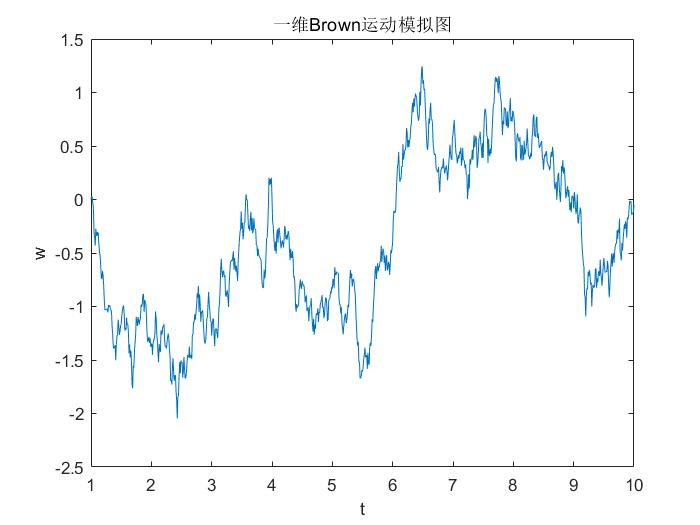
\includegraphics[width=8cm]{images/15.jpg}\\
  \caption{}\label{fig15}
\end{figure}



\section{布朗运动}
\textbf{定义:}概率空间$(\Omega,\mathcal{F},\mathbb{P})$上的随机过程$\{X(t),t\ge0\}$称为高斯过程,若对任意的$n\ge1,t_1,t+2,...,t_n,(X(t_1),...,X(t_n))$服从高斯分布。

\textbf{定理:}设$B=\{B(t),t\ge0\}$是零初值的实值随机过程。则它是布朗运动的充要条件是它是一个高斯过程,并且$\mathbb{E}(B(t))=0,\mathbb{E}(B(t)B(s))=t\wedge s=\min(s,t).$

\textbf{证明:}\textbf{必要性}。由独立增量性$n\ge1,t_1,t_2,...,t_n,(X(t_1),...,X(t_n))$服从高斯分布。又因为
\begin{equation}
\left(\begin{array}{c}B(t_1)\\
                      B(t_2)\\
                      \vdots\\
                      B(t_n)\end{array}\right)=\left(\begin{array}{ccccc}1&0&0&\cdots&0\\
                      1&1&0&\cdots&0\\
                      \vdots&\vdots&\vdots&\ddots&\vdots\\
                      1&1&1&\cdots&1\end{array}\right)\left(\begin{array}{c}B(t_1)\\
                      B(t_2)-B(t_1)\\
                      \vdots\\
                      B(t_n)-B(t_{n-1})\end{array}\right)
\end{equation}


\section{布朗运动}
 所以有$(B(t_1),...,B(t_n))$服从高斯分布。显然有$\mathbb{E}(B(t))=0,$对任意$t\ge s\ge0$,有
 \begin{equation}
 \mathbb{E}(B(t)B(s))=E(B(t)-B(s))B(s)+\mathbb{E}B^2(s)=s.
 \end{equation}

\textbf{充分性}。先证独立增量性。由于它们服从正态分布,所以只需要证明不相关性即可。事实上,对任意的$i<j$,有
\begin{equation}
\begin{split}
\mathbb{E}(B(t_i)-B(t_{i-1}))(B(t_j)-B(t_{j-1}))=&\mathbb{E}B(t_i)B(t_j)-\mathbb{E}B(t_{i-1})B(t_j)\\
                                                 &+\mathbb{E}B(t_{i-1})B(t_{j-1})\\
                                                 &=t_i-t_i-t_{i-1}+t_{i-1}=0.
\end{split}
\end{equation}
显然,对任意的$t>s,B(t)-B(s)$服从正态分布,均值为0,方差为
\begin{equation}
\mathbb{E}(B(t)-B(s))^2=\mathbb{E}B^2(t)-2\mathbb{E}B(t)B(s)+\mathbb{E}B^2(s)=t-s.
\end{equation}


\section{布朗运动的构造}
下面利用Fourier级数直接构造布朗运动。 假设$B$是一个标准布朗运动。定义过程$W(t)=B(t)-tB(1),t\in[0,1]$.称为$[0,1]$上的布朗桥。注意到$W(0)=W(1)=0$.我们将$W$在$[0,1]$上的Fourier展开($L^2$意义下)
 \begin{equation}
 W(t)=\sum_{n=1}^{\infty}X_nsin(n\pi t)
 \end{equation}
 其中系数$X_n$是随机变量,表达式为
 \begin{equation}
 X_n=2\int_0^tW(t)sin(n\pi t)dt.
 \end{equation}
 则$X_n$服从正态分布,可以计算
 \begin{equation}
 \mathbb{E}X_n=0,\mathbb{E}[X_nX_m]=\frac{2}{\pi^2n^2}\delta_{mn}.
 \end{equation}
 令$Z_0=B_1,Z_n=n\pi X_n/\sqrt{2},n\ge1.$ 则$\{Z_n\}$ i.i.d~$N(0,1)$。我们可以将布朗运动写成
 \begin{equation}
 B(t)=tZ_0+\frac{\sqrt{2}}{\pi}\sum_{j=1}^{\infty}\frac{Z_n}{n}sin(n\pi t),t\in[0,1].
 \end{equation}


\section{布朗运动的逼近}
三种逼近方式:

(1)基于随机游动的逼近;

(2)布朗运动的帕里-维纳表示;

(3)基于小波函数的逼近方法。


\section{布朗运动的应用}
金融数学:几何布朗运动是连续时间情况下的随机过程,其中随机变量的对数遵循布朗运动。用来在布莱克-舒尔斯定价模型中模仿股票价格。
\begin{figure}[H]
  \centering
  % Requires \usepackage{graphicx}
  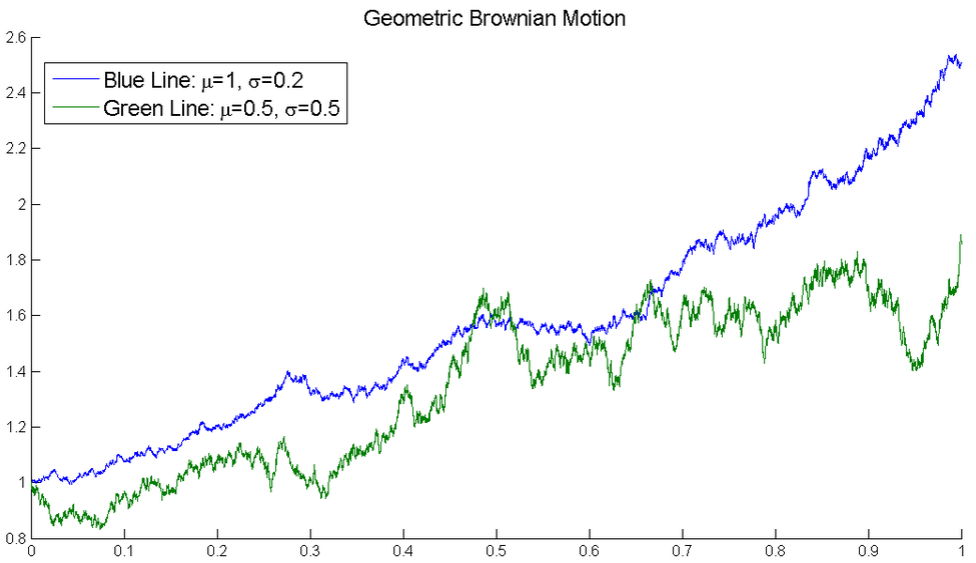
\includegraphics[width=8cm]{images/17.png}\\
  \caption{}\label{fig15}
\end{figure}


\section{布朗运动的应用}
使用几何布朗运动来描述股票价格的理由:
\begin{itemize}
  \item 几何布朗运动的期望与随机过程的价格(股票价格)是独立的, 这与我们对现实市场的期望是相符的。
  \item 几何布朗运动过程与我们在股票市场观察到的价格轨迹呈现了同样的“roughness” 。
  \item 几何布朗运动过程计算相对简单。
\end{itemize}

使用几何布朗运动来描述股票价格的缺陷:
\begin{itemize}
  \item 在真实股票价格中波动随时间变化, 但是在几何布朗运动中, 波动是不随时间变化的。
  \item 在真实股票价格中, 收益通常不服从正态分布。
\end{itemize}



\section{布朗运动的其他应用}
\begin{itemize}
  \item 研究仪器的灵敏度:在近代无线电技术 (如卫星通讯 ) 中,由于放大倍数很高,电涨落现象表现得特别显著,引起热噪声,这个问题也需要用布朗运动理论来研究。
  \item 研究各类扩散现象:扩散现象的本质是布朗运动产生的位移,因此布朗运动理论可用于各类扩散现象。例如半导体 中载流子 (电子或空穴 ) 的扩散,原子核反应堆中中子的扩散等,均可用布朗运动理论来研究。
  \item 分形布朗运动模型在地形分析、模式识别、数字图像处理、信息讯号的处理中的应用。
  \item 1990年以来,量子布朗运动理论进一步发展,转向对纳米结构中粒子运动和生物细胞中分子机器的研究。
\end{itemize}


\end{document}
